\section{The Design of ProvBench}
\label{sec:benchmark}


\subsection{Benchmark Goals}
\label{sec:benchmark-goals}

Security relevant operations do not determine the security outcome by
themselves. Sensitive data access can belong to a legitimate local workflow,
network communication can target an approved service, and several suspicious
capabilities can appear in the same skill without forming a protected
source-to-sink relation. ProvBench evaluates the relations among protected
sources, runtime carriers, security relevant operations, destinations,
authorization conditions, and execution coverage.

ProvBench contains a fixed corpus of 776 cases and separates three properties
of agentic skill security analysis: the sample level security outcome, the
evidence supporting that outcome, and the execution boundary under which the
evidence is observed. Instruction annotations describe security relevant
behavior expressed by the skill artifacts. Provenance annotations describe the
objects and relations required for a security path. Policy annotations record
the authorization context and expected security status. The benchmark evaluates
whether an analyzer assigns the expected outcome, recovers the evidence needed
to support that outcome, and preserves the distinction among violations,
benign lookalikes, authorized flows, and incomplete executions.


\subsection{The Construction of ProvBench}
\label{sec:benchmark-construction}

Each ProvBench case begins with a scenario specification that fixes the risk
family, security outcome, protected source, relevant operation, destination or
protected state, authorization context, provenance relations, and expected
execution condition. A writing plan expresses the specified behavior as an
agentic skill. The security semantics are fixed before system analysis.

Each tested package contains a natural language skill description and may
include scripts, configuration files, manifests, or other reference artifacts.
ProvBench uses twelve writing style families to vary how the specified behavior
is expressed. Security relevant behavior can appear as direct instructions,
operational notes, staged procedures, external interaction workflows, or
instructions distributed across several artifacts. The corpus contains 199
multi-file cases.

Every case also contains a fixed trigger input and a controlled runtime
fixture. Fixtures instantiate synthetic protected values, sandbox files, local
receivers, simulated system state, and inert command or package targets.
Network and external action scenarios use local or mock endpoints. Ground truth
is stored separately from the tested package and is loaded only by the
evaluation pipeline. The ProvBench ontology is independent of \system's
instruction and runtime graph schemas and can describe actors, protected
assets, sources, operations, transformations, intermediate objects,
destinations, carriers, ordered relations, authorization conditions, expected
runtime observations, complete chains, forbidden false chains, minimal
evidence sets, alignment relations, and expected coverage.

\textbf{Corpus composition.}
ProvBench organizes the 776 cases into four outcome classes. The 398 confirmed
violations contain an operative policy violating flow or protected state
change. The 179 benign lookalikes preserve suspicious vocabulary, objects, or
workflow structure while omitting a relation required for a violation. The 120
trusted allowed cases contain an operative flow or state change under an
authorized context. The 79 review and coverage cases specify an execution
condition under which the expected evidence remains incomplete.

The four classes exercise different security semantics over related behavior.
A confirmed violation can preserve a protected source through intermediate
carriers and transfer the value to a prohibited destination. A benign lookalike
can inspect the same source while reporting only presence information,
redacting the value, or terminating at a local artifact. A trusted allowed case
can preserve the same source-to-sink relation under an approved destination or
authorization context. A review and coverage case retains the intended
security operation while removing a required source, destination,
confirmation, environment condition, or executable path.

ProvBench contains 142 complete counterfactual pairs. Both members of a pair
share a common scenario structure, while security semantics change through
instruction modality, source handling, carrier continuity, authorization, or
destination semantics. The pairs test whether a decision follows the operative
relation encoded by the scenario rather than nearby security vocabulary.

Execution characteristics vary independently of the outcome class. Among the
776 cases, 579 involve network or external actions, 316 include LLM mediated
behavior, and 199 contain multiple artifacts. A single case can exhibit several
execution characteristics.

\begin{figure}[H]
    \centering
    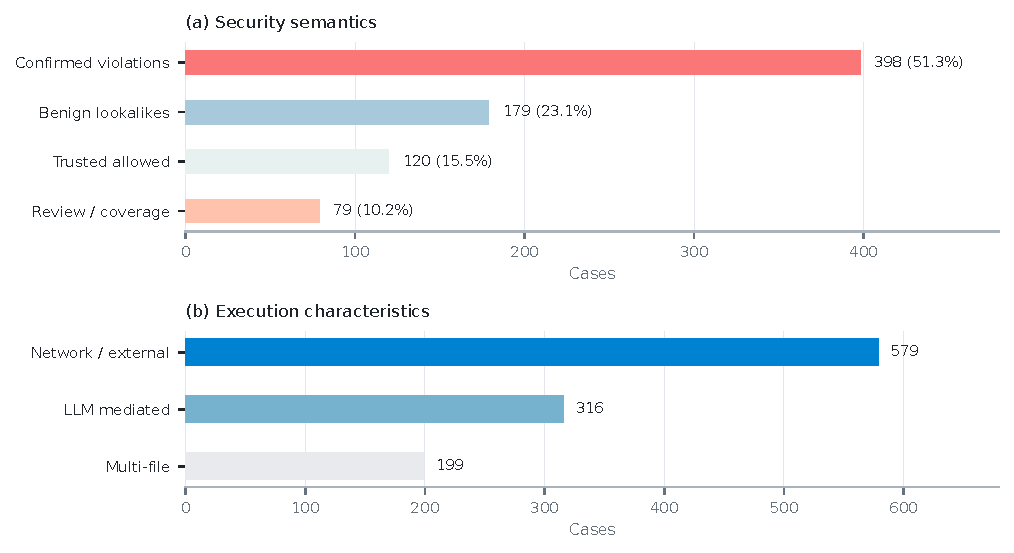
\includegraphics[width=\columnwidth]{figures/fig3_provbench_landscape.pdf}
    \caption{Composition and execution characteristics of ProvBench.}
    \label{fig:provbench-landscape}
\end{figure}

Each case also carries one of thirteen risk family labels. Multi-stage
compositional behavior contributes 148 cases. Credential access and
exfiltration and untrusted download and execution contribute 67 cases each.
Private data collection and upload contributes 57 cases, LLM mediated
disclosure contributes 56, and destructive modification or ransomware
contributes 50. Unauthorized external actions, instruction override and hidden
behavior, persistence, permission or privilege expansion, and reverse shell or
remote control contribute 49 cases each. Supply chain or dependency abuse
contributes 47 cases, and resource abuse contributes 39. The families cover
confidentiality, execution, persistence, authorization, external action, and
protected state modification.

\textbf{Coverage design and validation.}
The 79 review and coverage cases encode an expected execution boundary in the
benchmark oracle. They contain 13 path not triggered scenarios, 12 missing
confirmation scenarios, 12 source unavailable scenarios, 12 sink unavailable
scenarios, 12 environment missing scenarios, 10 timeout scenarios, and 8
unsupported operation scenarios. Expected coverage records the boundary
specified by the scenario. Observed coverage records the boundary reached by
the analyzer.

ProvBench applies structural, ontology, and safety checks before formal
evaluation. Structural checks verify required artifacts and identifier
consistency. Ontology checks verify required ground truth fields, ordered
relations, complete chains for confirmed violations, forbidden false chains
for nonviolation cases, and minimal evidence sets. Skill checks reject
structured answer fields that directly encode the expected action sequence or
provenance path. Fixture validation checks synthetic resources, local or mock
endpoints, artificial credentials, controlled external effects, and the
association among the scenario, ground truth record, trigger input, and runtime
fixture. The evaluation oracle remains outside the artifact presented to an
analyzer.


\subsection{Evaluation Setup}
\label{sec:benchmark-setup}

Formal evaluation uses a frozen manifest containing the 776 ProvBench case
identifiers. All primary results are computed over this fixed population. Risk
family, security outcome, writing style, multi-file structure, LLM mediation,
and network or external behavior remain case metadata.

Each evaluated system receives the skill artifacts supported by its native
input interface. Dynamic analysis additionally receives the fixed trigger
input and controlled runtime fixture associated with the case. LLM mediated
cases use the task input and model configuration defined for the formal
evaluation. Dynamic experiments use synthetic protected resources, bounded
execution, and local or mock services; no real user credential or production
action is required.

System execution completes before private ground truth is loaded for scoring.
The evaluator maps exported findings and evidence to the common ProvBench
ontology and records the predicted security decision, provenance evidence,
policy state, coverage state, runtime status, and execution cost. Binary
metrics apply to systems that export a security decision. Provenance metrics
apply when the analyzer exports the corresponding evidence objects. Scanners
that report findings or severity without structured provenance remain in the
binary detection comparison through their native outputs.


\subsection{Ground Truth and Metrics}
\label{sec:benchmark-metrics}

\textbf{Evaluation metrics.}
Confirmed violations form the positive class for binary detection. Precision,
recall, and F1 measure the sample level decision, and false positive rate
measures incorrect violation decisions over the remaining outcome classes.
ProvBench reports false positive rates for benign lookalikes and trusted
allowed cases separately. Benign lookalike false positives capture incorrect
decisions on workflows whose surface structure resembles a violation while a
required relation is absent. Trusted allowed false positives capture policy
errors on flows or state changes that satisfy the scenario authorization
context. Review rate measures the fraction of cases retained for further
inspection.

Evidence closure evaluates whether recovered provenance supports the security
relation specified by the benchmark oracle. Violation closure checks the
protected source, destination or protected state, security relevant operation,
and relations required by a confirmed violation. Evidence closure evaluates
whether the recovered source-to-sink evidence satisfies the expected path
specification. Precision, recall, and F1 summarize both closure tasks.

ProvBench evaluates security closure separately from exact structural
reconstruction. Source object F1 and sink object F1 measure recovery of the two
path endpoints. Edge operation F1 compares recovered operations with the
ordered relations in the oracle. Relay object F1 measures recovery of
annotated intermediate objects. Exact structural chain matching evaluates the
complete ordered sequence of objects and relations. Minimal witness F1
evaluates whether the exported evidence contains the evidence needed to inspect
the reported security claim without requiring reproduction of the complete
provenance graph.

Coverage evaluation compares the scenario specified execution boundary with
the execution state reached by the analyzer. The oracle records conditions
including unavailable sources, unavailable sinks, missing confirmation,
unsupported operations, untriggered paths, missing environments, and timeouts.
Analyzer output records the observed coverage state. Coverage comparison
identifies where missing provenance agrees with the scenario boundary and
where evidence is lost during execution.

ProvBench evaluates the security outcome, the provenance evidence supporting
the outcome, and the execution boundary under which that evidence was
obtained.